\documentclass[10pt]{article}
\usepackage{fullpage}
\usepackage{pgf}
\usepackage{tikz}
\usepackage[fleqn]{amsmath}
\usetikzlibrary{arrows,automata}
\usepackage{graphicx}
\usepackage{amssymb}
\usepackage{epstopdf}
\DeclareGraphicsRule{.tif}{png}{.png}{`convert #1 `dirname #1`/`basename #1 .tif`.png}
\pagestyle{empty}
\begin{document}
\thispagestyle{empty}

\setlength{\parindent}{0in}
\begin{center}
\textbf{\large Homework 1--CSC 320 Spring 2020}\\
\text{Mark Kaiser V00884677}

\end{center}

\bigskip

\begin{enumerate}


\item (20 {\sc Marks}) Let $L_1$ be  the set of strings over $\{a,b\}^*$ that contain at least two $a$'s
and $L_2$ be  the set of strings over $\{a,b\}^*$ that contain at most two $a$'s.
\begin{enumerate}
\item $L_1$ = $\{w \in \{a,b\}^* ~|~ |a| \le 2 \}$\\
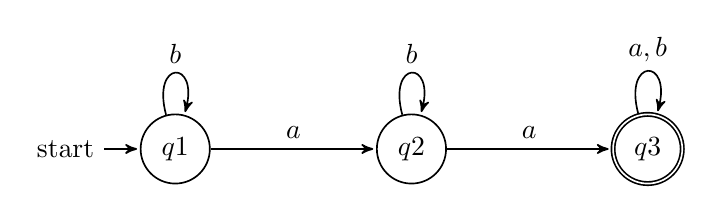
\begin{tikzpicture}[->,>=stealth',shorten >=1pt,auto,node distance=3cm,
                    semithick]

 \node[state](B)       {$q2$};
  \node[initial,state] (A)  [left of=B]                  {$q1$};
  \node[accepting,state](C) [right of=B]   	   {$q3$};
 

  \path (A) edge              node {$a$} (B)
            edge      [loop above]     node {$b$} (A)
           (B) edge [loop above] node {$b$} (A)
                edge              node {$a$} (C)
           (C) edge  [loop above] node {$a,b$} (C)
                ;

\end{tikzpicture}

\item $L_2$ = $\{w \in \{a,b\}^* ~|~ |a| \ge 2 \}$\\
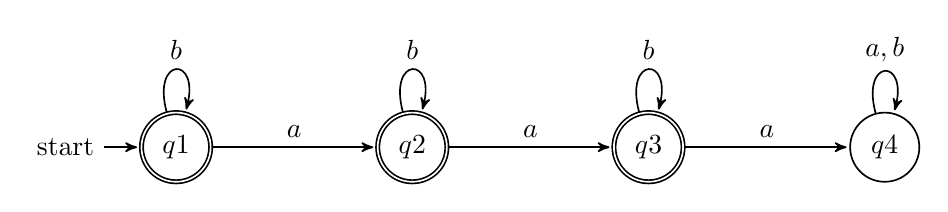
\begin{tikzpicture}[->,>=stealth',shorten >=1pt,auto,node distance=3cm,
                    semithick]

 \node[accepting,state](B)      				{$q2$};
  \node[initial,accepting,state] (A)  [left of=B]       {$q1$};
  \node[accepting,state](C) [right of=B]   	   	{$q3$};
  \node[state](D) [right of=C]				{$q4$};
 

  \path (A) edge              node {$a$} (B)
            edge      [loop above]     node {$b$} (A)
           (B) edge [loop above] node {$b$} (B)
                edge              node {$a$} (C)
	   (C) edge [loop above] node {$b$} (C)
                edge              node {$a$} (D)
           (D) edge  [loop above] node {$a,b$} (D)
                ;

\end{tikzpicture}

\item 
\[L_1 \cup L_2\]
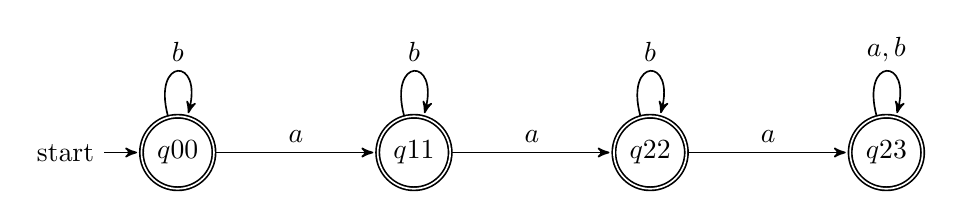
\begin{tikzpicture}[->,>=stealth',shorten >=1pt,auto,node distance=3cm,
                    semithick]

 \node[accepting,state](B)      				{$q11$};
  \node[initial,accepting,state] (A)  [left of=B]       {$q00$};
  \node[accepting,state](C) [right of=B]   	   	{$q22$};
  \node[accepting,state](D) [right of=C]		{$q23$};
 

  \path (A) edge              node {$a$} (B)
            edge      [loop above]     node {$b$} (A)
           (B) edge [loop above] node {$b$} (B)
                edge              node {$a$} (C)
	   (C) edge [loop above] node {$b$} (C)
                edge              node {$a$} (D)
           (D) edge  [loop above] node {$a,b$} (D)
                ;

\end{tikzpicture}

\end{enumerate}

\item (20 {\sc Marks}) Use the construction given in class to convert the following NFA to a DFA. Give a
transition table {\em and} a transition diagram for the resulting DFA.

\begin{center}
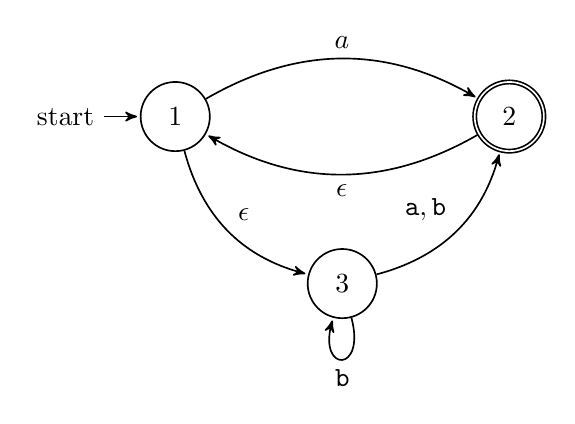
\begin{tikzpicture}[->,>=stealth',shorten >=1pt,auto,node distance=3cm,
                    semithick]

 \node[state](C)       {$3$};
  \node[initial,state] (A)  [above left of=C]                  {$1$};
  \node[accepting,state](B) [above right of=C]   	   {$2$};
 

  \path (A) edge   [bend left]           node {$a$} (B)
            edge      [bend right]     node {$\epsilon$} (C)
           (B) edge [bend left] node {$\epsilon$} (A)
                
           (C) edge  [bend right] node {$\mathtt{a,b}$} (B)
           (C) edge [loop below] node {$\mathtt{b}$} (C)
                ;

\end{tikzpicture}
\end{center}
\begin{table}[h]
\begin{tabular}{lll}
          & a         & b         \\
\{1,3\}   & \{1,2,3\} & \{1,2,3\} \\
\{1,2,3\} & \{1,2,3\} & \{1,2,3\}
\end{tabular}
\end{table} 
\begin{center}
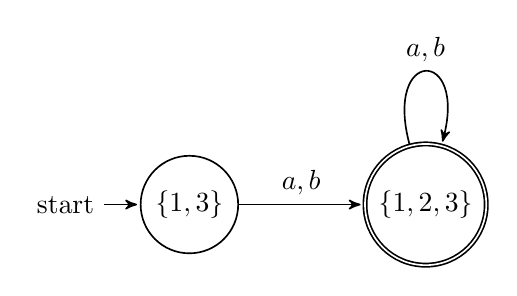
\begin{tikzpicture}[->,>=stealth',shorten >=1pt,auto,node distance=3cm,
                    semithick]

  \node[initial,state] (A)                 			{$\{1,3\}$};
  \node[accepting,state](B) [right of=A]   	   	{$\{1,2,3\}$};
 

  \path (A) edge           		node {$a,b$} (B)
           (B) edge [loop above] 	node {$a,b$} (A)
                ;

\end{tikzpicture}
\end{center}

\item (20 {\sc Marks}) Use the procedure given in class to convert the following regular expression
to an NFA
\[
(((\mathtt{00})^*(\mathtt{11}))\cup\mathtt{01})^*
\]
\[R = 0\]
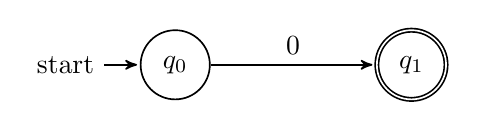
\begin{tikzpicture}[->,>=stealth',shorten >=1pt,auto,node distance=3cm,
                    semithick]

  \node[initial,state] (A)                 			{$q_0$};
  \node[accepting,state](B) [right of=A]   	   	{$q_1$};
 

  \path (A) edge           		node {$0$} (B)
                ;

\end{tikzpicture} \\
\[R = 1\]
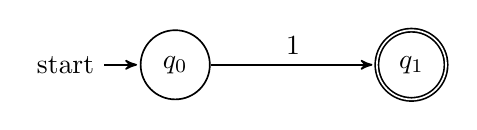
\begin{tikzpicture}[->,>=stealth',shorten >=1pt,auto,node distance=3cm,
                    semithick]

  \node[initial,state] (A)                 			{$q_0$};
  \node[accepting,state](B) [right of=A]   	   	{$q_1$};
 

  \path (A) edge           		node {$1$} (B)
                ;

\end{tikzpicture} \\
\[R = \mathtt{00}\]
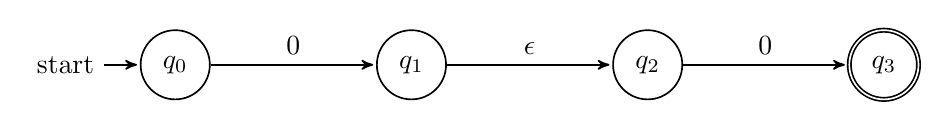
\begin{tikzpicture}[->,>=stealth',shorten >=1pt,auto,node distance=3cm,
                    semithick]

  	\node[initial,state] (A)                 			{$q_0$};
  	\node[state](B) [right of=A]   	   			{$q_1$};
	\node[state](C) [right of=B]   	   			{$q_2$};
	\node[accepting,state](D) [right of=C]   	   	{$q_3$};
 

  	\path (A) edge           		node {$0$} (B);
	\path (B) edge         	  		node {$\epsilon$} (C);
	\path (C) edge           		node {$0$} (D);

\end{tikzpicture} \\
\[R = \mathtt{11}\]
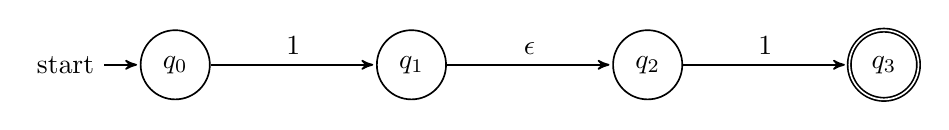
\begin{tikzpicture}[->,>=stealth',shorten >=1pt,auto,node distance=3cm,
                    semithick]

  	\node[initial,state] (A)                 			{$q_0$};
  	\node[state](B) [right of=A]   	   			{$q_1$};
	\node[state](C) [right of=B]   	   			{$q_2$};
	\node[accepting,state](D) [right of=C]   	   	{$q_3$};
 

  	\path (A) edge           		node {$1$} (B);
	\path (B) edge         	  		node {$\epsilon$} (C);
	\path (C) edge           		node {$1$} (D);

\end{tikzpicture} \\
\[R = \mathtt{01}\]
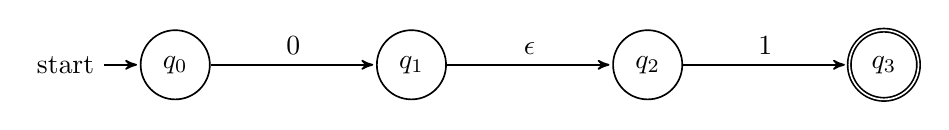
\begin{tikzpicture}[->,>=stealth',shorten >=1pt,auto,node distance=3cm,
                    semithick]

  	\node[initial,state] (A)                 			{$q_0$};
  	\node[state](B) [right of=A]   	   			{$q_1$};
	\node[state](C) [right of=B]   	   			{$q_2$};
	\node[accepting,state](D) [right of=C]   	   	{$q_3$};
 

  	\path (A) edge           		node {$0$} (B);
	\path (B) edge         	  		node {$\epsilon$} (C);
	\path (C) edge           		node {$1$} (D);

\end{tikzpicture} \\
\[R = (\mathtt{00})^*\]
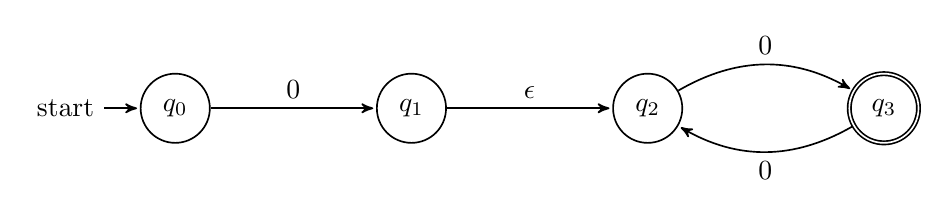
\begin{tikzpicture}[->,>=stealth',shorten >=1pt,auto,node distance=3cm,
                    semithick]

  	\node[initial,state] (A)                 			{$q_0$};
  	\node[state](B) [right of=A]   	   			{$q_1$};
	\node[state](C) [right of=B]   	   			{$q_2$};
	\node[accepting,state](D) [right of=C]   	   	{$q_3$};
 

  	\path (A) edge           		node {$0$} (B);
	\path (B) edge         	  		node {$\epsilon$} (C);
	\path (C) edge  [bend left] 		node {$0$} (D);
	\path (D) edge  [bend left]		node {$0$} (C);

\end{tikzpicture} \\
\[R = (\mathtt{00})^*(\mathtt{11})\]
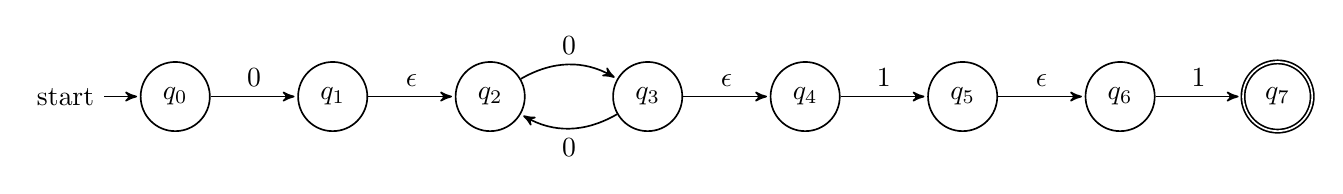
\begin{tikzpicture}[->,>=stealth',shorten >=1pt,auto,node distance=2cm,
                    semithick]

  	\node[initial,state] (A)                 			{$q_0$};
  	\node[state](B) [right of=A]   	   			{$q_1$};
	\node[state](C) [right of=B]   	   			{$q_2$};
	\node[state](D) [right of=C]   	   			{$q_3$};
	\node[state](E) [right of=D]   	   			{$q_4$};
	\node[state](F) [right of=E]   	   			{$q_5$};
	\node[state](G) [right of=F]   	   			{$q_6$};
	\node[accepting,state](H) [right of=G]   	   	{$q_7$};
 

  	\path (A) edge           		node {$0$} (B);
	\path (B) edge         	  		node {$\epsilon$} (C);
	\path (C) edge  [bend left] 		node {$0$} (D);
	\path (D) edge  [bend left]		node {$0$} (C);
	\path (D) edge         	  		node {$\epsilon$} (E);
	\path (E) edge         	  		node {$1$} (F);
	\path (F) edge         	  		node {$\epsilon$} (G);
	\path (G) edge         	  		node {$1$} (H);

\end{tikzpicture} \\\\\\
\[R = ((\mathtt{00})^*(\mathtt{11}))\cup\mathtt{01}\]
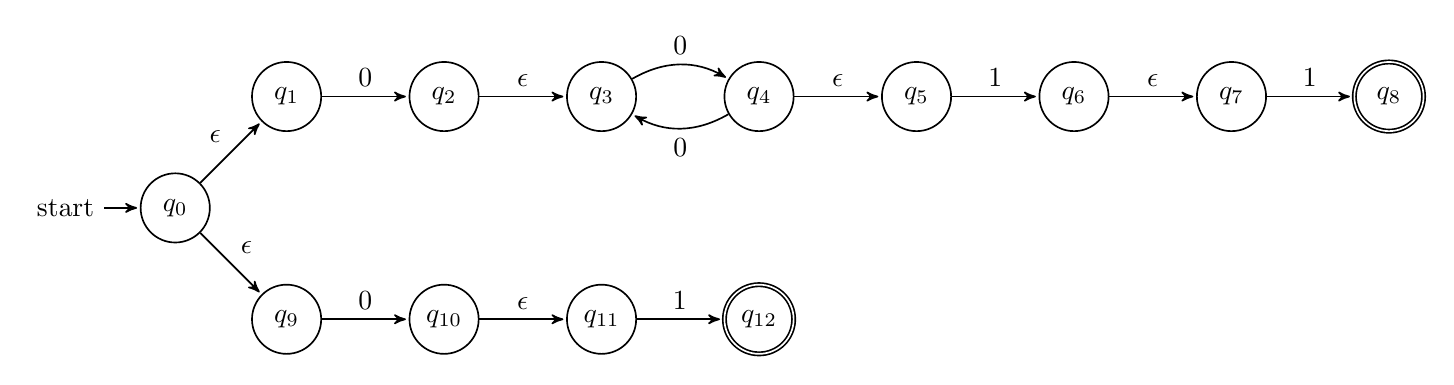
\begin{tikzpicture}[->,>=stealth',shorten >=1pt,auto,node distance=2cm,
                    semithick]

  	\node[initial,state] (a)                 			{$q_0$};
  	\node[state](A) [above right of=a]   	   		{$q_1$};
  	\node[state](B) [right of=A]   	   			{$q_2$};
	\node[state](C) [right of=B]   	   			{$q_3$};
	\node[state](D) [right of=C]   	   			{$q_4$};
	\node[state](E) [right of=D]   	   			{$q_5$};
	\node[state](F) [right of=E]   	   			{$q_6$};
	\node[state](G) [right of=F]   	   			{$q_7$};
	\node[accepting,state](H) [right of=G]   	   	{$q_8$};

  	\node[state](I) [below right of=a]                	{$q_9$};
  	\node[state](J) [right of=I]   	   			{$q_{10}$};
	\node[state](K) [right of=J]   	   			{$q_{11}$};
	\node[accepting,state](L) [right of=K]   	   	{$q_{12}$};
 

	\path (a) edge         	  		node {$\epsilon$} (A);
  	\path (A) edge           		node {$0$} (B);
	\path (B) edge         	  		node {$\epsilon$} (C);
	\path (C) edge  [bend left] 		node {$0$} (D);
	\path (D) edge  [bend left]		node {$0$} (C);
	\path (D) edge         	  		node {$\epsilon$} (E);
	\path (E) edge         	  		node {$1$} (F);
	\path (F) edge         	  		node {$\epsilon$} (G);
	\path (G) edge         	  		node {$1$} (H);

	\path (a) edge         	  		node {$\epsilon$} (I);
  	\path (I) edge        	   		node {$0$} (J);
	\path (J) edge         	  		node {$\epsilon$} (K);
	\path (K) edge           			node {$1$} (L);

\end{tikzpicture} \\
\[R = (((\mathtt{00})^*(\mathtt{11}))\cup\mathtt{01})^*\]
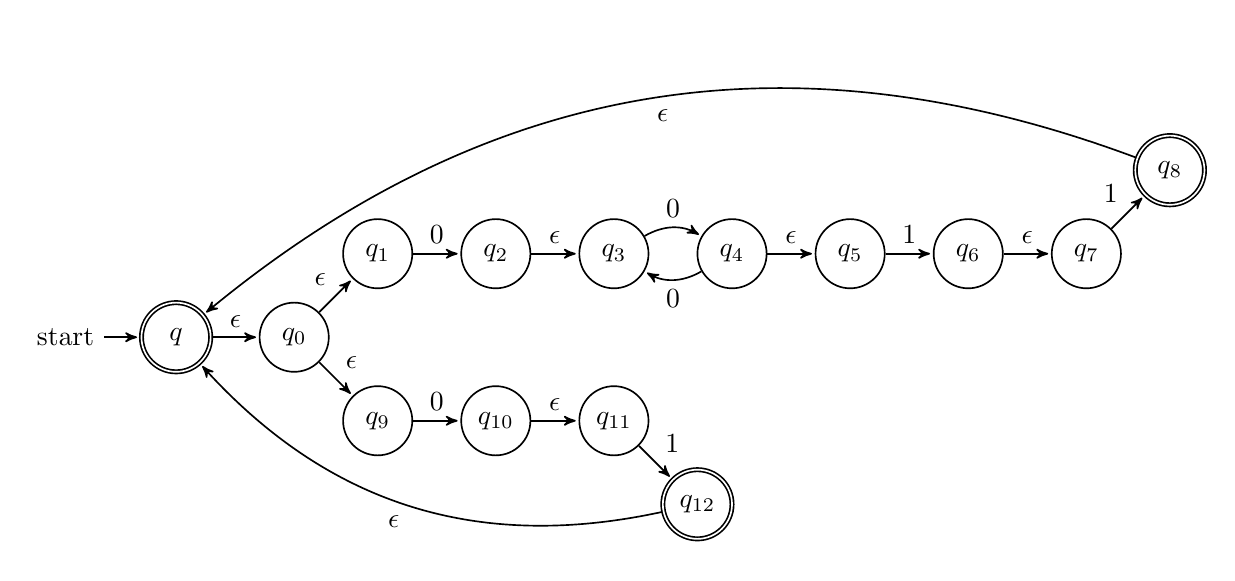
\begin{tikzpicture}[->,>=stealth',shorten >=1pt,auto,node distance=1.5cm,
                    semithick]

  	\node[initial,accepting,state] (a)                 		{$q$};
  	\node[state] (aa) [right of=a]                 		{$q_0$};
  	\node[state](A) [above right of=aa]   	   		{$q_1$};
  	\node[state](B) [right of=A]   	   			{$q_2$};
	\node[state](C) [right of=B]   	   			{$q_3$};
	\node[state](D) [right of=C]   	   			{$q_4$};
	\node[state](E) [right of=D]   	   			{$q_5$};
	\node[state](F) [right of=E]   	   			{$q_6$};
	\node[state](G) [right of=F]   	   			{$q_7$};
	\node[accepting,state](H) [above right of=G]   	{$q_8$};

  	\node[state](I) [below right of=aa]                	{$q_9$};
  	\node[state](J) [right of=I]   	   			{$q_{10}$};
	\node[state](K) [right of=J]   	   			{$q_{11}$};
	\node[accepting,state](L) [below right of=K]  	{$q_{12}$};
 

	\path (a) edge         	  		node {$\epsilon$} (aa);
	\path (aa) edge         	  		node {$\epsilon$} (A);
  	\path (A) edge           		node {$0$} (B);
	\path (B) edge         	  		node {$\epsilon$} (C);
	\path (C) edge  [bend left] 		node {$0$} (D);
	\path (D) edge  [bend left]		node {$0$} (C);
	\path (D) edge         	  		node {$\epsilon$} (E);
	\path (E) edge         	  		node {$1$} (F);
	\path (F) edge         	  		node {$\epsilon$} (G);
	\path (G) edge         	  		node {$1$} (H);

	\path (aa) edge         	  		node {$\epsilon$} (I);
  	\path (I) edge        	   		node {$0$} (J);
	\path (J) edge         	  		node {$\epsilon$} (K);
	\path (K) edge           			node {$1$} (L);

	\path (H) edge   [bend right]	node {$\epsilon$} (a);
	\path (L) edge	[bend left]       	node {$\epsilon$} (a);

\end{tikzpicture} \\
\item (20 {\sc Marks}) Use the procedure given in class to convert the following DFA to a regular expression
\begin{center}
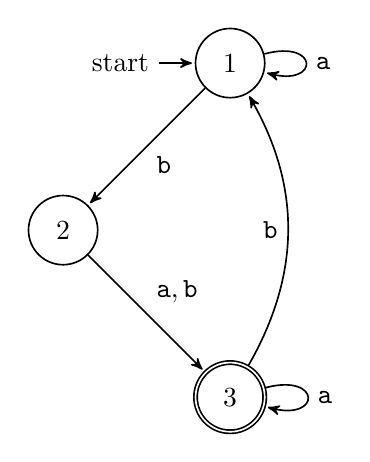
\begin{tikzpicture}[->,>=stealth',shorten >=1pt,auto,node distance=3cm,
                    semithick]

 \node[initial,state](C)       {$1$};
\node[state] (B) [below left of = C] {$2$};
\node[accepting,state] (A)  [below right of =B]       {$3$};
  
 

  \path (C) edge   [loop right] node {$\mathtt{a}$} (C)
               edge                   node {$\mathtt{b}$} (B)
          (B) edge                  node  {$\mathtt{a,b}$} (A)      
          (A) edge  [loop right] node {$\mathtt{a}$} (A)
               edge  [bend right] node {$\mathtt{b}$} (C); 


\end{tikzpicture} \newpage
\end{center}
GNFA:\\
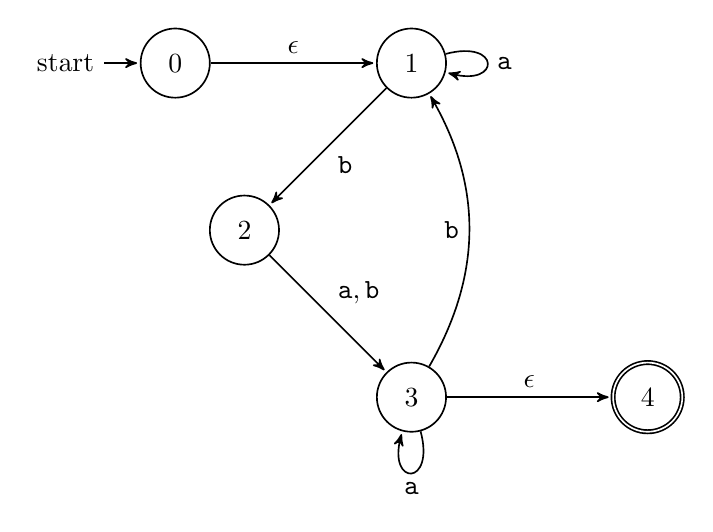
\begin{tikzpicture}[->,>=stealth',shorten >=1pt,auto,node distance=3cm,
                    semithick]

\node[initial,state](A)       {$0$};
\node[state](B) [right of=A]      {$1$};
\node[state] (C) [below left of=B] {$2$};
\node[state] (D)  [below right of=C]       {$3$};
\node[accepting,state] (E)  [right of =D]       {$4$};
  
  \path 
	(A) edge node {$\epsilon$} (B)
	(B) edge   [loop right] node {$\mathtt{a}$} (B)
               edge                   node {$\mathtt{b}$} (C)
          (C) edge                  node  {$\mathtt{a,b}$} (D)      
          (D) edge  [loop below] node {$\mathtt{a}$} (D)
               edge  [bend right] node {$\mathtt{b}$} (B)
		edge 		node {$\epsilon$} (E);
\end{tikzpicture} \\

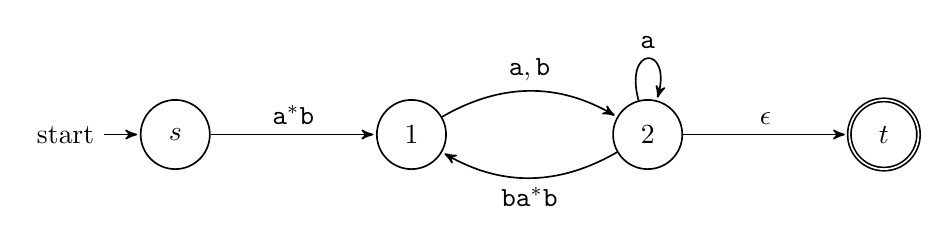
\begin{tikzpicture}[->,>=stealth',shorten >=1pt,auto,node distance=3cm,
                    semithick]

  	\node[initial,state] (A)                 			{$s$};
  	\node[state](B) [right of=A]   	   			{$1$};
	\node[state](C) [right of=B]   	   			{$2$};
	\node[accepting,state](D) [right of=C]   	   	{$t$};
 

  	\path (A) edge           		node {$\mathtt{a^*b}$} (B);
	\path (B) edge [bend left]  		node {$\mathtt{a,b}$} (C);
	\path (C) edge [bend left]  		node {$\mathtt{ba^*b}$} (B);
	\path (C) edge [loop above]  	node {$\mathtt{a}$} (C);
	\path (C) edge           		node {$\epsilon$} (D);

\end{tikzpicture} \\

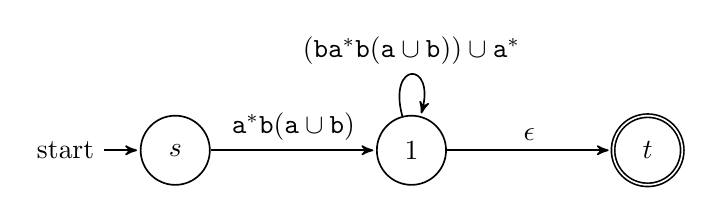
\begin{tikzpicture}[->,>=stealth',shorten >=1pt,auto,node distance=3cm,
                    semithick]

  	\node[initial,state] (A)                 			{$s$};
  	\node[state](B) [right of=A]   	   			{$1$};
	\node[accepting,state](C) [right of=B]   	   	{$t$};
 

  	\path (A) edge           		node {$\mathtt{a^*b(a \cup b)}$} (B);
	\path (B) edge		  		node {$\epsilon$} (C);
	\path (B) edge [loop above]  	node {$\mathtt{(ba^*b(a \cup b)) \cup a^*}$} (B);

\end{tikzpicture} \\

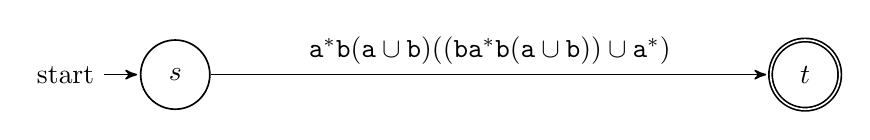
\begin{tikzpicture}[->,>=stealth',shorten >=1pt,auto,node distance=8cm,
                    semithick]

  	\node[initial,state] (A)                 			{$s$};
	\node[accepting,state](B) [right of=A]   	   	{$t$};
 

  	\path (A) edge           		node {$\mathtt{a^*b(a \cup b)((ba^*b(a \cup b)) \cup a^*)}$} (B);

\end{tikzpicture} \\

\item 
Assume the languages A and B are regular.  Take the interleave of A with B, $A \wr B$.  We want to show that $A \wr B$ is regular.  The interleave of A and B $A \wr B$ gives:
\[
w=a_1b_1a_2b_2\dots a_kb_k \mbox{ where } a_1\dots a_k \in A, b_1 \dots b_k \in B \mbox { and } a_i \in \Sigma^a, b_i \in \Sigma^b, 1 \le i \le k\
\]
We construct the interleave of $A \wr B$ by concatenating $k \ge 1$ (not necessarily distinct) sets of strings, $a_i$, $b_i$, where $1 \le i \le k$.  $a_i$ and $b_i$ are constructed by machines $M_a$ and $M_b$ respectively.  We can form the interleave by concatenating $a_i$ with $b_i$ for $k$ times.  Since we can construct a machine that accepts the interleave of A and B, given that A and B are both regular, then $A \wr B$ is also regular.
\end{enumerate}


\end{document}  